\documentclass[letterpaper]{sig-alternate-05-2015}


%~~~~~~~~~~~~~~~~~~~~~~~~~~~~~~~~~~~~~~~~~~~~~~~~~~~~~~~~~~~~~~~~~~~~~~~~~~~~~~~~~~~~~~~~~~~~~~~~~~~~~~~

\usepackage{graphicx}
\usepackage{hyperref} %[hidelinks] to hide hyperlinks
\usepackage[utf8]{inputenc}
\usepackage[normalem]{ulem}
\usepackage{slashbox}
\usepackage{color,soul} %Highlighting

%Timestamp on bottom
\usepackage[scrtime]{prelim2e}


%----------------------------------------------------------------------------------

% rename autorefnames
\def\sectionautorefname{Section}
\def\subsectionautorefname{Section}
\def\subsubsectionautorefname{Section}
\def\figureautorefname{Figure}
\def\tableautorefname{Table}

\usepackage{units}
\usepackage{siunitx}
\DeclareSIUnit\wn{\raiseto{-1}\cm}
\sisetup{
range-phrase = --,
range-units = single,
list-units = single,
product-units = single,
list-final-separator = {, and },
}


\usepackage{glossaries}
\makeglossaries
\newacronym{IoT}{IoT}{Internet of Things}
\newacronym{NFC}{NFC}{Near Field Communications}
\newacronym{RFID}{RFID}{Radio Frequency Identification}
\newacronym{DTW}{DTW}{Dynamic Time Warping}
\newacronym{HMM}{HMM}{Hidden Markov Model}
\newacronym{SVM}{SVM}{Support Vector Machine}
\newacronym{k-NN}{k-NN}{K-Nearest Neighbor}
\newacronym{ANN}{ANN}{Artificial Neural Networks}
\usepackage{notoccite}

\sloppy

%~~~~~~~~~~~~~~~~~~~~~~~~~~~~~~~~~~~~~~~~~~~~~~~~~~~~~~~~~~~~~~~~~~~~~~~~~~~~~~~~~~~~~~~~~~~~~~~~~~~~~~~


\begin{document}

\doi{XXXX}
\isbn{XXXX}

\title{Gesture-Based Peer-to-Peer Pairing Authentication for Assymmetric \glsentrylong{IoT} Devices}

\numberofauthors{3} 
\author{
% 1st. author
\alignauthor
Joe Chen\\
       \email{joe.chen@rice.edu}
 % 2nd author
 \alignauthor
Zilong (Gino) Liao\\
       \email{zl15@rice.edu}
 % 3rd author
\alignauthor
Heng-Yi (Henry) Lin\\
       \email{henry.hy.lin@rice.edu}
}

\maketitle
\begin{abstract}
\input{chapters/abstract}
\end{abstract}

%!TEX root = ../iotpaper.tex

\section{Introduction}
\label{sec:Introduction}

In an \gls{IoT} environment, mobile devices may need to pair or authenticate themselves to other devices. However, unlike the traditional internet, an \gls{IoT} environment does not typically have a centralized certificate authority, making it difficult for one device to determine if another device is authentic. Furthermore, these \gls{IoT} devices are often resource-constrained, meaning traditional cryptographic defenses that support confidentiality, integrity, and authenticity difficult to implement \cite{cisco:iot-pf,authmodels}.

One potential solution to this problem is to use biometrics---especially motion and gestures---in order to validate the identity of the device. Prior work has shown that impostors has a low probability of imitating a gesture calibrated to another person successfully \cite{Casanova}. Furthermore, motion recognition is suitable for \gls{IoT} systems which feature small sensors and low powered devices because motion recognition can achieve high accuracy with just an accelerometer \cite{RuizeXu}. 

Some prior work have looked at motion sensor data fusion across different devices to detect pairing, for example detecting device collision when tiling two tablets together \cite{SyncGes}. Existing work in gesture recognition and event detection focuses on gestures on the same device or similar devices (e.g. two tablets, gestures on a Wiimote \cite{LiuuWave}). However, pairing in an \gls{IoT} environment is usually needed for two asymmetric devices with different types of hardware sensors (e.g. a smartwatch with a smartphone).

In this project, we analyze the use of gestures as a biometric for peer-to-peer authentication in an \gls{IoT} scenario, where sensor devices are asymmetric. 

\section{Attack \& Defense Models}
\label{sec:Attacks}

Our project analyzes the following three key defense models for authentication.

\begin{itemize}
\item \emph{Model 1:} This system model contains three entities: a legitimate prover, a verifier, and an attacker. The legitimate prover is non-malicious and wants to pair with the verifier. Both the legitimate prover and the verifier are owned by the same person (e.g. a smartphone and a smartwatch). However, the attacker is a malicious prover and wants to also pair with the verifier. To distinguish between the attacker and legitimate prover, the verifier uses gesture recognition to distinguish between the two parties. 

\begin{figure}[!tb]
\centering
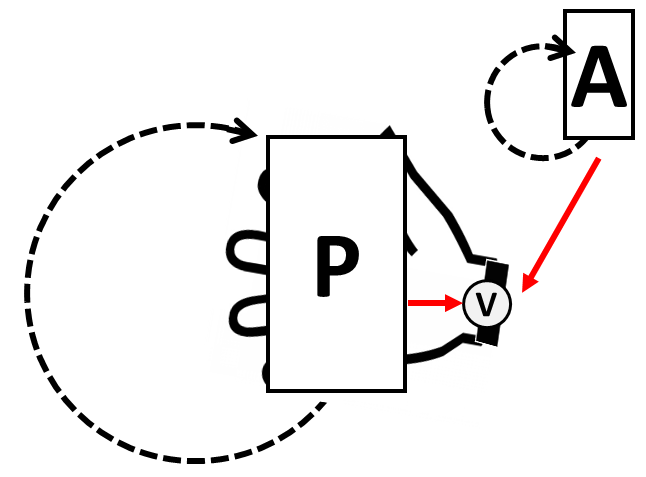
\includegraphics[width=0.65 \linewidth]{./figures/model1.png}
\caption{System model for defense model 1. The verifier (V) and the prover (P) are synchronized in motion. The attacker (A) must try to mimic the motion of the verifier in order to trick the system.}
\label{fig:Model1}
\end{figure}

Since the legitimate prover and verifier are owned by the same person, the user performs any generic gesture while holding both devices as shown in \autoref{fig:Model1}. Accelerometer data is used to read the gesture, and a matching gesture authenticates the prover.

In contrast, the attacker must mimic the gesture of the verifier in order to trick the verifier. Our hypothesis is that we can keep false negatives (rejecting legitimate provers) and false positives (accepting attackers) to less than 10\%. This is modest compared to existing works due to the hardware asymmetry.  

\item \emph{Model 2:} This system model contains the same three entities as in Model 1. In this model, the verifier has previously calibrated a single secret gesture with the user that is needed to pair with the device as shown in \autoref{fig:Model2}. Devices that want to pair with the verifier must produce accelerometer data that matches this gesture with no prior knowledge about the gesture. Since this gesture is a predefined secret, only the prover needs to collect accelerometer data during the proof of authenticity.

\begin{figure}[!tb]
\centering
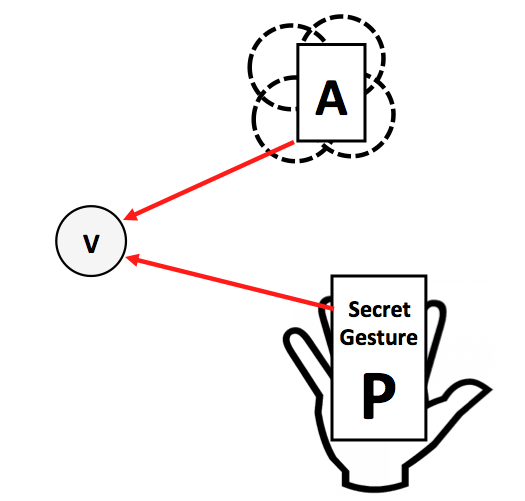
\includegraphics[width=0.6 \linewidth]{./figures/model2.png}
\caption{System model for defense model 2. The verifier (V) and the prover (P) are not synchronized in motion, and the verifier has previously established a secret gesture for pairing. The attacker (A) can brute force a gesture if it has no knowledge of the secret gesture, or it may imitate a gesture that it sees that a legitimate prover used.}
\label{fig:Model2}
\end{figure}

An attacker may try to trick this model in the following two ways. First, if no information about the secret gesture has been leaked to the attacker, it will attempt a brute force attack and attempt several common gesture shapes, such as a circle, line, or even just shaking the device. Second, an attacker may learn information about which gesture is the secret gesture by watching a legitimate prover validate themselves to the verifier. These visual clues then reveal what the actual gesture is, and the attacker scenario reduces to the same as in Model 1. 

For the second attack, we hypothesize that we will again achieve less than 10\% false negatives for legitimate provers. However, we hypothesize 0\% false positives for attackers if the secret gesture is not within the library of brute force attempts (i.e. the gesture recognition algorithm works). 

\item \emph{Model 3:} The final model once again contains the same three entities as the prior models. Although similar to Model 2, this model establishes a pre-defined library of gestures at the verifier previously calibrated by the user. During the pairing process, the verifier will challenge the prover to a subset of the gesture library. As shown in \autoref{fig:Model3}, the verifier sends visual prompts about what the gestures should be during the challenge process (i.e. the library of gestures is public). However, to trick the system, an attacker must produce the gesture in the same way as the intended user. 

\begin{figure}[!tb]
\centering
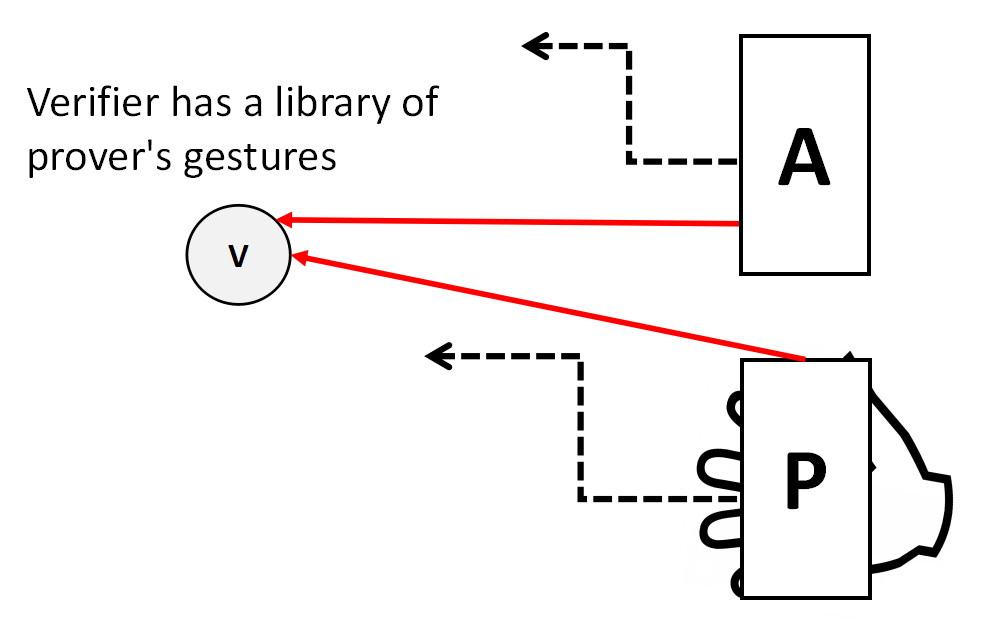
\includegraphics[width=0.65 \linewidth]{./figures/model3.png}
\caption{System model for defense model 3. The verifier (V) and the prover (P) are not synchronized in motion, and the verifier challenges the prover with a series of gestures in its pre-calibrated library. The attacker (A) receives the same prompts, but must mimic what the prover would do for each gesture.}
\label{fig:Model3}
\end{figure}

We hypothesize that there is a inverse correlation between number of gesture challenges and number of false positives (i.e. more challenges reduces the success of an attacker. However, we also hypothesize there is a direct correlation between number of gesture challenges and number of false negatives (i.e. there are more opportunities for the user to fail). We seek to find a threshold that minimizes the number of false positives and false negatives in this model.

\end{itemize}


%!TEX root = ../iotpaper.tex

\section{Attack \& Defense Models}
\label{sec:Attacks}

Our project analyzes the following two key defense models for authentication.

\begin{itemize}
\item \emph{Simultaneous Gesture Model:} This system model contains three entities: a legitimate prover, a verifier, and an attacker. The legitimate prover is non-malicious and wants to pair with the verifier. Both the legitimate prover and the verifier are owned by the same person (e.g. a smartphone and a smartwatch). However, the attacker is a malicious prover and wants to also pair with the verifier. To distinguish between the attacker and legitimate prover, the verifier uses gesture recognition to distinguish between the two parties. 

\begin{figure}[!tb]
\centering
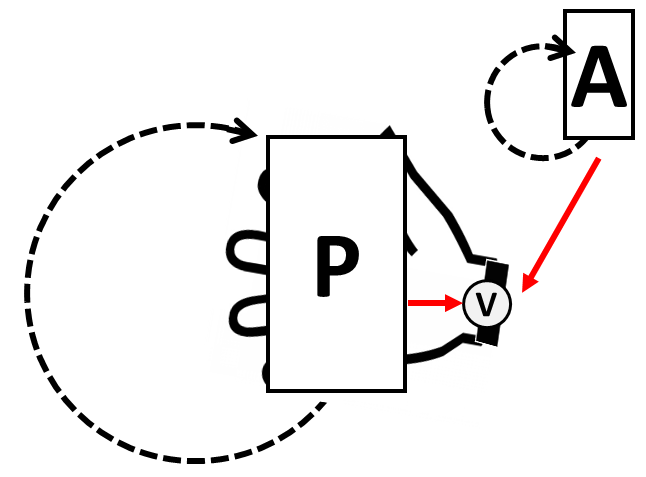
\includegraphics[width=0.65 \linewidth]{./figures/model1.png}
\caption{System model for the Simultaneous Gesture defense model. The verifier (V) and the prover (P) are synchronized in motion. The attacker (A) must try to mimic the motion of the verifier in order to trick the system.}
\label{fig:Model1}
\end{figure}

Since the legitimate prover and verifier are owned by the same person, the user performs any generic gesture while holding both devices as shown in \autoref{fig:Model1}. Accelerometer data is used to read the gesture, and a matching gesture authenticates the prover.

In contrast, the attacker must mimic the gesture of the verifier in order to trick the verifier. Our hypothesis is that we can keep false negatives (rejecting legitimate provers) and false positives (accepting attackers) to less than 10\%. This is modest compared to existing works due to the hardware asymmetry.  

%\item \emph{Secret Gesture Model:} This system model contains the same three entities as in the Simultaneous Gesture defense model. In this model, the verifier has previously calibrated a single secret gesture with the user that is needed to pair with the device as shown in \autoref{fig:Model2}. Devices that want to pair with the verifier must produce accelerometer data that matches this gesture with no prior knowledge about the gesture. Since this gesture is a predefined secret, only the prover needs to collect accelerometer data during the proof of authenticity.

%\begin{figure}[!tb]
%\centering
%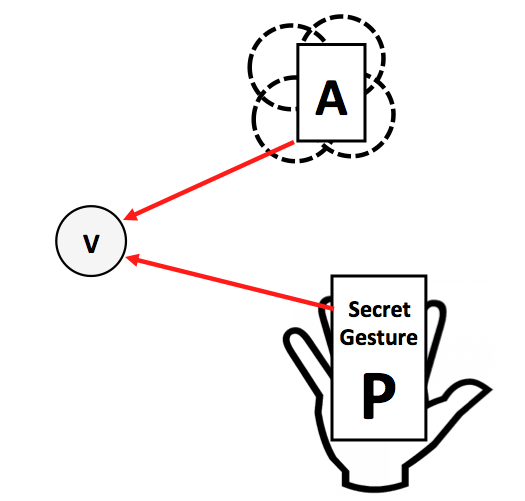
\includegraphics[width=0.6 \linewidth]{./figures/model2.png}
%\caption{System model for defense model 2. The verifier (V) and the prover (P) are not synchronized in motion, and the verifier has previously established a secret gesture for pairing. The attacker (A) can brute force a gesture if it has no knowledge of the secret gesture, or it may imitate a gesture that it sees that a legitimate prover used.}
%\label{fig:Model2}
%\end{figure}
%
%An attacker may try to trick this model in the following two ways. First, if no information about the secret gesture has been leaked to the attacker, it will attempt a brute force attack and attempt several common gesture shapes, such as a circle, line, or even just shaking the device. Second, an attacker may learn information about which gesture is the secret gesture by watching a legitimate prover validate themselves to the verifier. These visual clues then reveal what the actual gesture is, and the attacker scenario reduces to the same as in Model 1. 
%
%For the second attack, we hypothesize that we will again achieve less than 10\% false negatives for legitimate provers. However, we hypothesize 0\% false positives for attackers if the secret gesture is not within the library of brute force attempts (i.e. the gesture recognition algorithm works). 

\item \emph{Gesture Library Model:} The final model has the same three entities. The user has already successfully paired one device with the verifier and sent training data of a library of gestures to the verifier. This library of gestures is collected at the already-paired device and simply stored at the verifier. In order to pair a new device to the verifier, the prover must recreate these gestures with the new device.

%In particular, we address the case where the legitimate user hasThe library may collect user's same gesture from different devices, because of one possible scenario that user may change pairing device over time and we want the user to be able to pair with the verifier even though the pairing device is different. 
During the pairing process, the verifier will challenge the prover to a subset of the gesture library. As shown in \autoref{fig:Model3}, the verifier sends visual prompts about what the gestures should be during the challenge process (i.e. the library of gestures is public). However, to trick the system, an attacker must produce the gesture in the same way as the intended user. The attacker may use the same device as the user or different devices. Even with device asymmetry, we want attacker to be denied and the actual user to be authenticated. 

\begin{figure}[!tb]
\centering
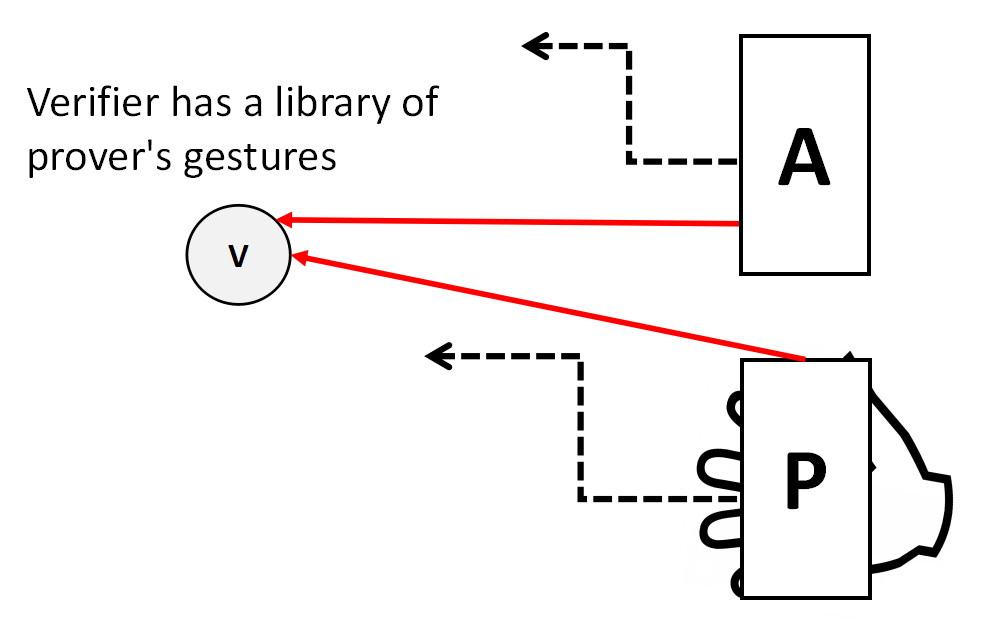
\includegraphics[width=0.65 \linewidth]{./figures/model3.png}
\caption{System model for the gesture library defense model. The verifier (V) and the prover (P) are not synchronized in motion, and the verifier challenges the prover with a series of gestures in its pre-calibrated library. The attacker (A) receives the same prompts, but must mimic what the prover would do for each gesture.}
\label{fig:Model3}
\end{figure}

We hypothesize that there is a inverse correlation between number of gesture challenges and number of false positives (i.e. more challenges reduces the success of an attacker. However, we also hypothesize there is a direct correlation between number of gesture challenges and number of false negatives (i.e. there are more opportunities for the user to fail). We seek to find a threshold that minimizes the number of false positives and false negatives in this model.

\end{itemize}


%!TEX root = ../iotpaper.tex

\subsection{Experimental Platform}
\label{sec:Tooling}

Our experiments focus on multiple mobile devices with 3-axis accelerometers: two iPhone 6, one iPhone 6s, Nexus 5 (Android). For ease of implementation, each device communicates with a laptop running MATLAB, and the laptop takes and compares the accelerometer data from each device. We also compare performance against a classic Pebble smartwatch's accelerometer data. The data flow is shown in \autoref{fig:hardware}.

\begin{figure}[!tb]
\centering
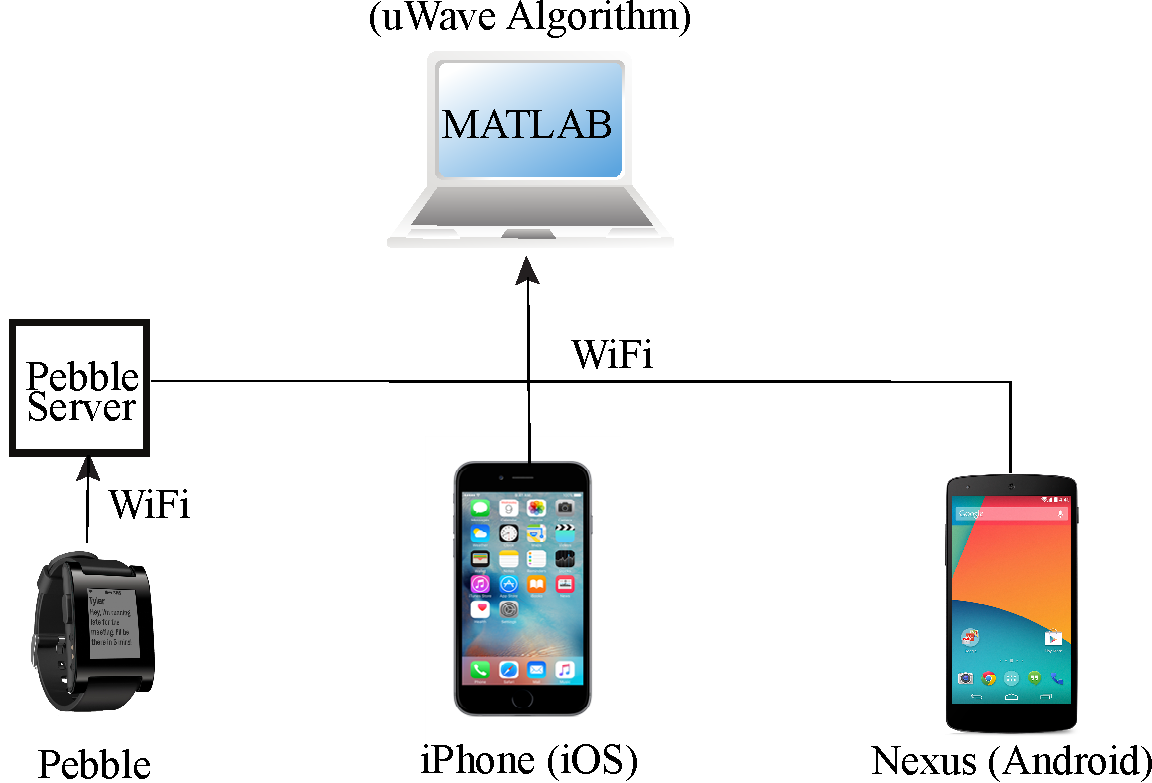
\includegraphics[width=0.9 \linewidth]{./figures/hardware_composition.pdf}
\caption{The hardware setup for the gesture-based authentication experiments. The iPhone and Android connect to MATLAB via WiFi. The Pebble smartwatch stores its data on a 3rd party server. The data is retrieved via WiFi and then imported into MATLAB.}
\label{fig:hardware}
\end{figure}

The iPhone and Nexus devices communicate with MATLAB via WiFi through the MATLAB sensor hardware support package (iOS\footnote{http://www.mathworks.com/hardware-support/iphone-sensor.html} and Android\footnote{http://www.mathworks.com/hardware-support/android-sensor.html}). The Pebble smartwatch records its accelerometer data using one of its 1st party applications called XXXXXX. The application sends the accelerometer data to an online server, and we download the data and compare the results against the iPhone/Nexus results in MATLAB. Both the smartwatch and the cellular devices are timestamped, so we line up the timestamps to reduce the impact of data desync on our experiments for Model 1: simultaneous gesture authentication. 

For gesture recognition, we implement uWave \cite{Liu:2009, LiuuWave}, which was developed in the Rice Efficient Computing Group. The algorithm uses \gls{DTW} to obtain the distance between two time series accelerometer data to characterize how closely two gestures match. Their algorithm simplifies the time series data such that even simple 16-bit microcontroller can do the computation. The uWave authors have provided their original source code in C, and we have converted the gesture recognition modules into MATLAB implementations. 

We set each accelerometer to sample as quickly as the hardware allows us to sample---one sample per 100\,ms for the iPhone devices, one sample per 20\,ms for the Android device, and one sample per 40\,ms for the Pebble smartwatch. Because these are relatively slow sampling rates, we choose not to apply any smoothing to the accelerometer data. 

%%!TEX root = ../iotpaper.tex

\section{Progress}
\label{sec:Progress}

\subsection{Current Accomplishments}

\begin{itemize}
\item Successfully extracted accelerometer data from all three mobile devices
\item Basic gesture functionality of uWave converted to MATLAB programming environment.
\item Initial distance measurements between non-malicious and malicious provers for gesture recognition on a signle device.
\end{itemize}

\subsection{Future Milestones}

\begin{itemize}
\item \emph{April 6:} Rigorous Model 3 experiments completed. Scripting for Model 1 completed (remove axis/orientation bias).
\item \emph{April 13:} Rigorous Model 1 \& 2 testing completed. 
\item \emph{April 22:} Finalize project report/conduct follow up experiments. 
\item \emph{Final Exam Period:} Final project presentation
\end{itemize}

\subsection{Generalized Division of Labor}

\begin{itemize}
\item \emph{Joe:} Lead for MATLAB software development and wiimote integration.
\item \emph{Zilong:} Lead for Android software development. 
\item \emph{Heng-Yi:} Lead for iOS software development. 
\end{itemize}


%%!TEX root = ../iotpaper.tex

\section{Experimental Results}
\label{sec:Results}


\subsection{Gesture Recognition on a Single Device}
At first, we want to test our assumption that there are enough difference between time samples of the same gesture performed by different users. So all three team members performs the same gesture with the same iPhone device.

The current data includes 10 samples of writing letter `e' by Gino, 1 sample of writing letter `s', `e' by all three members. All accelerometer data are stores as `.mat' file and each one comes with a plot of acceleration on `x', `y', `z' axes versus time. The time length of each data file depends on how long the user finishes the gesture. The start time and end time of capturing data depend on user.

Then, we performs uWave algorithm. We first quantized the acceleration data, calculated the distance between two time samples and do dynamic time wraping to check if two gestures match. In our experiment, Gino is the original user and Joe and Henry are the attackers. Table~\ref{table:distanceOnSingleDevice} shows our result of distances to standard deviation of three users.

\begin{table}

\begin{center}
  \begin{tabular}{ c | c | c}
    \hline
    \backslashbox{Pairer}{Gesture}
      & Letter `e' & Letter `s' \\ \hline
    Gino & 5 & 6 \\ \hline
    Joe & 8 & 9 \\	\hline
    Henry & 8 & 9 \\
    \hline
  \end{tabular}
\end{center}
\caption{Distance to calibrated original time sample} % title of Table
\label{table:distanceOnSingleDevice}
\end{table}


 


%!TEX root = ../iotpaper.tex

%~~~~~~~~~~~~~~~~~~~~~~~~~~~~~~~~~~~~~~~~~~~~~~~~~~~~~~~~~~~~~~~


\section{Gesture Library Experiments}
\label{sec:GestureLibrary}

\begin{table}

\begin{center}
  \begin{tabular}{ c | c | c | c  }
    \hline
    1 & 2 & 3 & 4  \\ \hline
    
\includegraphics[width=0.2\linewidth, height=15mm]{./figures/gesture_e.png} & 
    
\includegraphics[width=0.2\linewidth, height=15mm]{./figures/gesture_s.png} &
    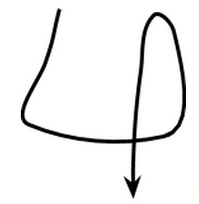
\includegraphics[width=0.2\linewidth, height=15mm]{./figures/gesture_num4.png} &
    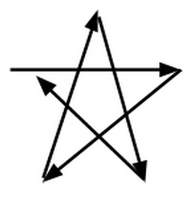
\includegraphics[width=0.2\linewidth, height=15mm]{./figures/gesture_star.png}  \\ \hline
    5 & 6 & 7 & 8 	 \\ \hline
    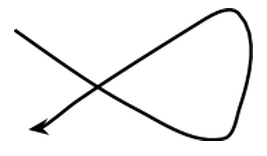
\includegraphics[width=0.2\linewidth, height=15mm]{./figures/gesture_5.png} &
    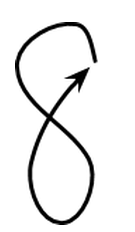
\includegraphics[width=0.2\linewidth, height=15mm]{./figures/gesture_num8.png} &
    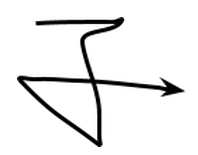
\includegraphics[width=0.2\linewidth, height=15mm]{./figures/gesture_7.png} &
    
\includegraphics[width=0.2\linewidth, height=15mm]{./figures/gesture_su.png}  \\ \hline
    9 & 10 & 11 & 12  \\ \hline
    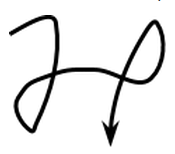
\includegraphics[width=0.2\linewidth, height=15mm]{./figures/gesture_mi.png} & 
    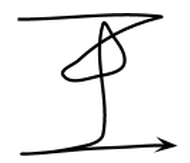
\includegraphics[width=0.2\linewidth, height=15mm]{./figures/gesture_wang.png} &
    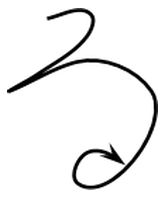
\includegraphics[width=0.2\linewidth, height=15mm]{./figures/gesture_ru.png} &
    
\includegraphics[width=0.2\linewidth, height=15mm]{./figures/gesture_miu.png}	\\ \hline
    13 & 14 & 15 & 16  \\ \hline
    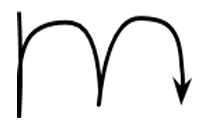
\includegraphics[width=0.2\linewidth, height=15mm]{./figures/gesture_m.png} &
    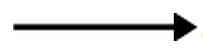
\includegraphics[width=0.2\linewidth, height=15mm]{./figures/gesture_14.png} &
    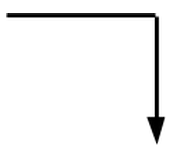
\includegraphics[width=0.2\linewidth, height=15mm]{./figures/gesture_15.png} & 
    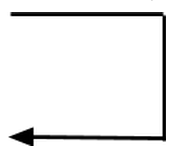
\includegraphics[width=0.2\linewidth, height=15mm]{./figures/gesture_16.png}  \\ \hline
    17    \\ \hline
    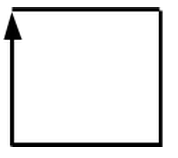
\includegraphics[width=0.2\linewidth, height=15mm]{./figures/gesture_17.png} \\ \hline
  \end{tabular}
\end{center}
\caption{Gestures for authentication} % title of Table
\label{table:GestureTable}
\end{table}


To test the Gesture Library Model, we collect gesture data from all three group members. Our experimental library consists of the 17 different gestures shown in \autoref{tab:GestureTable}. These gestures are a mix of European characters, Asian characters, and simple shapes, each with varying complexity. 

Gino is the legitimate user who performed calibration on his iPhone 6 device. To emulate a strong attacker, Henry attempts authentication using a second iPhone 6 device. Joe is a weaker attacker who attempts authentication on an iPhone 6s. Joe is less familiar with Asian characters, and thus is weaker than Henry because of the selecting gestures. Gino also attempts authentication on his second device, the Nexus 5, as a legitimate user.

For each gesture, Gino takes 30 calibration attempts on his iPhone 6. Afterwards, everyone attempts 10 new authentications for each gesture each day. In the next sections, we discuss calibration and set thresholds that minimize false negatives (rejecting Gino, the legitimate user), while also minimizing false positives (accepting Henry or Joe, the attackers).

\subsection{Calibration Mechanism}

Our calibration mechanism is a brute force search that calculates the \gls{DTW} distance of one attempt time series to another for the same gesture. The calibrated time series selected is the attempt with the smallest average distance to all of the other attempts. This approach is non-scalable ($O(N^{2})$ where $N$ is the number of calibration attempts). However, scalability is not the focus of this project because we can make calibration a one-time event at the beginning and choose not to update the history for the purposes of this experiment. For calibration, we use the full 30 attempts per gesture data set unless otherwise noted.

\subsection{Gesture Distance Consistency}

First, to prove that gesture-based authentication works, we monitor the consistency of the \gls{DTW} from the calibration time series over the period of 7 days for both the legitimate user and the attackers. We hypothesize that the average distance for all the attempts for a single gesture on a single day from the attackers stays at least one standard deviation away from the average distance for the intended user. Furthermore, we hypothesize that the intended user's average distance should stay within one standard deviation of the previous day's average.

\hl{DATA HERE}

\subsection{Threshold Setting}

\subsubsection{Technique}

The threshold for rejecting or accepting a user can be set using a variety of techniques. For this project, we use a simple threshold ($D_{t}$) based on the calibration data above as a proof of concept. Each attempt from calibration has an average \gls{DTW} distance from all of the other calibration attempts. Based on this distance, we can set a threshold tailored to gesture $i$ using \autoref{eq:thres}

\begin{equation}
D_{t} = m \cdot d_{i} + \frac{1.96 \cdot \delta_{i}}  {\sqrt{N}}
\label{eq:thres}
\end{equation}

\noindent where $m$ is a constant multiplicative factor, $d_{i}$ is a mean distance value based on the distance data from calibration for gesture $i$, and $\delta_{i}$ is the associated standard deviation.

Intuition suggests that choosing the minimum recorded \gls{DTW} distance for $d_{i}$ yields an overly strict system that minimizes false positives but also introduces additional false negatives to the system. Likewise, choosing the maximum recorded \gls{DTW} distance for $d_{i}$ produces an overly lenient system that minimizes false positives but introduces false negatives. 

To make the system more usable, we opt to split the difference to minimize both false positives and false negatives. However, if we must choose between more false positives and false negatives, we choose to err on the side of more false positives to make the system more usable to the end user. Therefore, we set $d_{i}$ based on the 80th, 85th, and 90th percentiles of the calibration data. This lets us minimize the effects of any major calibration outliers while still being lenient. Furthermore, the multiplicative factor $m$ is used to introduce some additional leniency because of day-to-day variation in the intended user's gesture. $m$ is varied from 1 to 5 in steps of 0.25.

Our hypothesis is that we can set an authentication distance threshold that keeps the false positives and false negatives rates averaged over all gestures below 10\% for all gestures.

\subsubsection{Results}

The optimal threshold settings are the ones that minimize both the false positives and false negatives. \autoref{fig:ThresFig} shows the results for false positives and false negatives for the (a) 80th, (b) 85th, and (c) 90th percentiles. For readability, we only include. $m$ values of 2, 2.5, and 3 in this figure.

\hl{Talk about the plots here}.

\subsection{Number of Calibration Iterations}

Thus far, our evaluation is based on our full data set of 30 calibration attempts per gesture. In this section, we investigate the performance of our Gesture Library model for smaller subsets of calibration attempts: 5, 15, and 30. We hypothesize that we will have more false positives and false negatives for the same parameters because of the smaller data set.

\hl{DATA HERE}.

\subsection{Multi-Attempt Authentication}

Placeholder

%~~~~~~~~~~~~~~~~~~~~~~~~~~~~~~~~~~~~~~~~~~~~~~~~~~~~~~~~~~~~~~~
 


%!TEX root = ../iotpaper.tex

%~~~~~~~~~~~~~~~~~~~~~~~~~~~~~~~~~~~~~~~~~~~~~~~~~~~~~~~~~~~~~~~


\section{Simultaneous Gestures \\ Experiments}
\label{sec:Simultaneous}

\subsection{Co-Located Devices}

\subsection{Not Co-Located Devices}


%~~~~~~~~~~~~~~~~~~~~~~~~~~~~~~~~~~~~~~~~~~~~~~~~~~~~~~~~~~~~~~~
 


%!TEX root = ../iotpaper.tex

\section{Related Work}
\label{sec:RelatedWork}

Our related work is divided into three key categories: (1) gesture recognition algorithms and implementations on a single accelerometer device, (2) device pairing via accelerometer data, and (3) other biometric recognition authentication techniques.

%!TEX root = ../iotpaper.tex

\subsection{Gesture \& Motion Recognition on a Single Device}

Several efficient gesture-recognition algorithms already exist. Jiayang et al. \cite{Liu:2009, LiuuWave} presented an algorithm called uWave that is based on a single accelerometer. uWave quantizes the acceleration data to reduce computational load and uses dynamic time warping(DTW) to measure similarities between two time series of accelerometer data. Template adaptation deals with gesture variation over the time. Ahmad and Shahrokh \cite{Ahmad:2010} also proposes a gesture recognition system that uses only one 3-axis accelerometer. The system temporally compresses the acceleration time series to filter out variations not intrinsic to the gesture itself and reduces the size of the acceleration signals for next step of dynamic time warping. Then, the system uses affinity propagation to find a good set of exemplars from all data points. Finally, they implemented compressive sensing to recognize a repetition of a gesture. 

For the best user experience, gesture recognition should be in real-time and easy to use. Instead of using a button to indicate start time and end time of a gesture motion, Zoltan \cite{Zoltan} proposes an automatic segmentation method and uses two classification algorithms: Hidden Markov Models(HMM) and Support Vector Machine to to give high accuracy. This system has great performance and low response time, thus a good model for \gls{IoT} devices.

Considering the quadratic time and space complexity with DTW algorithm and the need of larger training sets with HMM, Zhe Ji et al. \cite{Ji:2015} proposed a new algorithm which uses FastDTW instead of DTW and HMM. Their algorithm is divided into two part: preprocess and classification. In the preprocessing step, the raw data is first filtered by a series of low-pass filters and its amplitude is normalized. Then, it is resampled to a fixed length. After preprocessing the raw data, FastDTW, which has linear time and space complexity, is used to calculated the alignment between two time series. Their work shows that the performance drop is not necessary and is avoidable while replacing lightweight FastDTW to DTW for reducing computational demand.

%!TEX root = ../iotpaper.tex

\subsection{Device Pairing via Sensor Data}

In addition to recognition of a gesture, gesture-detection can also be used as a form of multifactor authentication to pair two separate devices together. Hinckley proposed one of the earlier forms of synchronous gesture authentication. By detecting an impulse when two tablets are pushed together, Hinckley pairs the two tablets, allowing the user to tile both devices together as one large screen \cite{SyncGes}. Vinteraction uses a combination of accelerometer and vibrator data to transmit private data between two devices in physical contact. The vibrations serve as the secret shared channel between the two devices \cite{vinteraction}. Mayrhofer et. al. have a user hold two mobile devices and shake randomly to establish a shared secret key. The shaking motion produces enough entropy to create a key that is difficult to predict \cite{ShakeWell}.

Jiang et. al. propose near-field vibration (NFV) to group multiple devices together at once. By propagating the vibrations of a smartphone through a table on which all group devices are placed, the smartphone can automatically pair with all of the devices in the group \cite{Jiang2016}. 

In a non-security based scenario, Duet explores combining sensor information for both a smartphone and a paired watch to create more sophisticated controls based on hand gestures \cite{Duet}. PickRing compares gyroscope data across a ring and a gyroscope to detect when a user picks up a smart device. However, the authors do not analyze the security of this approach against a malicious prover \cite{Wolf:2015}.

%!TEX root = ../iotpaper.tex

\subsection{Other Biometric Recognition Authentication Techniques}

Besides motion and gesture, various biometric characteristics could also be used for recognition as Jain et al. \cite{Jain} specified. These characteristics include: DNA, ear, face, facial thermogram, hand thermogram, hand vein, fingerprint, gait, hand geometry, iris, palmprint, retina, signature, and voice. In some applications, biometric traits are further exploited for machine-to-machine recognition authentication instead of conventional personal recognition.

One example of this idea is an authentication scheme based on heartbeat data (ECG) proposed by Rostami et al.\cite{Rostami:2013} It requires that the controller of implantable medical devices (IMDs) contacts the patient's body to control the IMD. Specifically, the controller can only gain access to IMDs if the ECG readings on the both devices are approximately the same.  
 
Furthermore, a patent \cite{Apple:2014} submitted by Apple Inc. depicts a more general authentication scheme using biometric data for wireless pairing and communication between devices. The scheme is simply based on the comparison of biometric data which received and stored by the device or the host. Thus, it is applicable with any sort of distinctive biometric traits for machine-to-machine authentication once they embed related module targeting to any specific trait on their commercial devices.   
%!TEX root = ../iotpaper.tex

\section{Conclusion \& Future Work}
\label{sec:Conclusion}

%Summarize contributions/key results 
Authentication without a central authority can be tricky, but biometrics can be one valuable factor for authentication without that resource. In this paper, we have shown that authentication with gestures has the potential to validate a user. In the Gesture Library model, we show that it is difficult to imitate most gestures and set a simple threshold for authentication based on a previously calibrated library. Although we are not able to reduce both false positives and false negatives to less than 10\%, we can control the equilibrium point by changing the number of challenges by the verifier. In the Simultaneous Gestures model, we have shown that copying a gesture visually---even with prior knowledge of what the gesture will be---is difficult, and the distance is typically one order of magnitude larger than the distance of the legitimate user if he holds the prover and verifier together. 

In the future, we recommend dynamically updating calibration data with new authentications so that the calibration data does not become stagnant. A threshold algorithm also needs to be set for the Simultaneous Gestures model, potentially one that extracts information about the time and complexity of the gesture itself.

%Future work
%-Dynamically update calibration based on historical information.
%-Threshold setting for the simultaneous gestures case (involves time and complexity)

\nocite{*} 
\bibliographystyle{abbrv}
\bibliography{iotsources}



\end{document}
